\chapter{Implementação}
\noindent

\paragraph{} A implementação do projeto começou com a instalação de um \textit{driver} RNDIS para microcontroladores da família STM32 ARM Cortex M4, sendo que para a implementação dessa etapa, se utilizou como base uma biblioteca criada pelo projeto Cobra 2020 da IMBEL \citep{cobra} licenciada para fins acadêmicos, que permite que o sistema do VANT possa interfacear com o modem RF, através de uma porta USB e \textit{drivers} de rede do sistema operacional, já que a referida interface é instalada pelo \textit{driver} RNDIS do SO (\textit{driver} presente nos sistemas operacionais Windows, Android e na maioria das distribuições Linux) como uma interface de rede comum. Isso foi feito para que a camada de aplicação pudesse interagir com a rede ad hoc em alto nível, de maneira genérica, da mesma forma como os celulares Android fazem ancoragem de rede USB. 

\paragraph{} A implementação ainda forneceu um servidor HTTP para configuração dos parâmetros da rede ad hoc e depuração da rede, de tal forma que essa configuração fosse feita através do navegador de um dispositivo conectado à rede.

\paragraph{} Dentro do microcontrolador foi instalada a biblioteca de código aberto da Nest \textit{Openthread} que recebe os \textit{frames} \textit{ethernet} IPv6 da camada RNDIS e faz o endereçamento dos pacotes, através do \textit{header} da subcamada MAC. Os pacotes passaram por um filtro inicial que seleciona os que são direcionados ao servidor HTTP, e não são transmitidos ao resto da rede. 

\paragraph{} Depois de passarem pela camada do \textit{OpenThread}, os pacotes foram fracionados, utilizando a biblioteca de código aberto RF24 \textit{Ethernet} que gerencia o fracionamento de até 1500 bytes em pacotes curtos de 20 bytes, que serão diretamente transmitidos pelo modem RF.

\paragraph{} Os pacotes de 20 bytes passam ainda pelo tratamento de inserção de códigos FEC, que transformam pacotes de 20 bytes em pacotes de 32 bytes, utilizando o algoritmo BCH.

\paragraph{} Para o projeto, foi elaborado um programa em linguagem C, que aplica o BCH em uma mensagem de 16 bits. Para que fosse possível enviar essa mensagem, foram introduzidos 47 bits de paridade, que gerou um código final de 63 bits. A codificação para ser do tipo \textit{“Narrow sense”} (ótima), exige uma distância de \textit{Hamming} de tamanho 23, assim podendo corrigir até 11 erros na palavra código. Para maior segurança, foi feita uma nova codificação para o projeto, a codificação de \textit{Reed-Solomon}, que também é capaz de corrigir até 11 erros em uma palavra código de 63 símbolos, porém usando apenas 22 símbolos de paridade. 

\paragraph{} Os pacotes de 32 bytes são enviados para a camada de controle do rádio nRF24L01+ que funciona em modo de transmissão \textit{broadcast} sem ACK. Em um único canal pré selecionado. Esse pacote entrega informações sobre a potência média do canal e o RSSI de cada transmissão. Para ser \textit{complience} com o protocolo IEEE 802.15.4, a estrutura de quadros utilizada pelo modem nRF24L01+ foi ajustada para se adequar a estrutura de quadro descrita no protocolo, conforme figura \ref{fig:figura80}.

\begin{figure}[!ht]
	\centering
	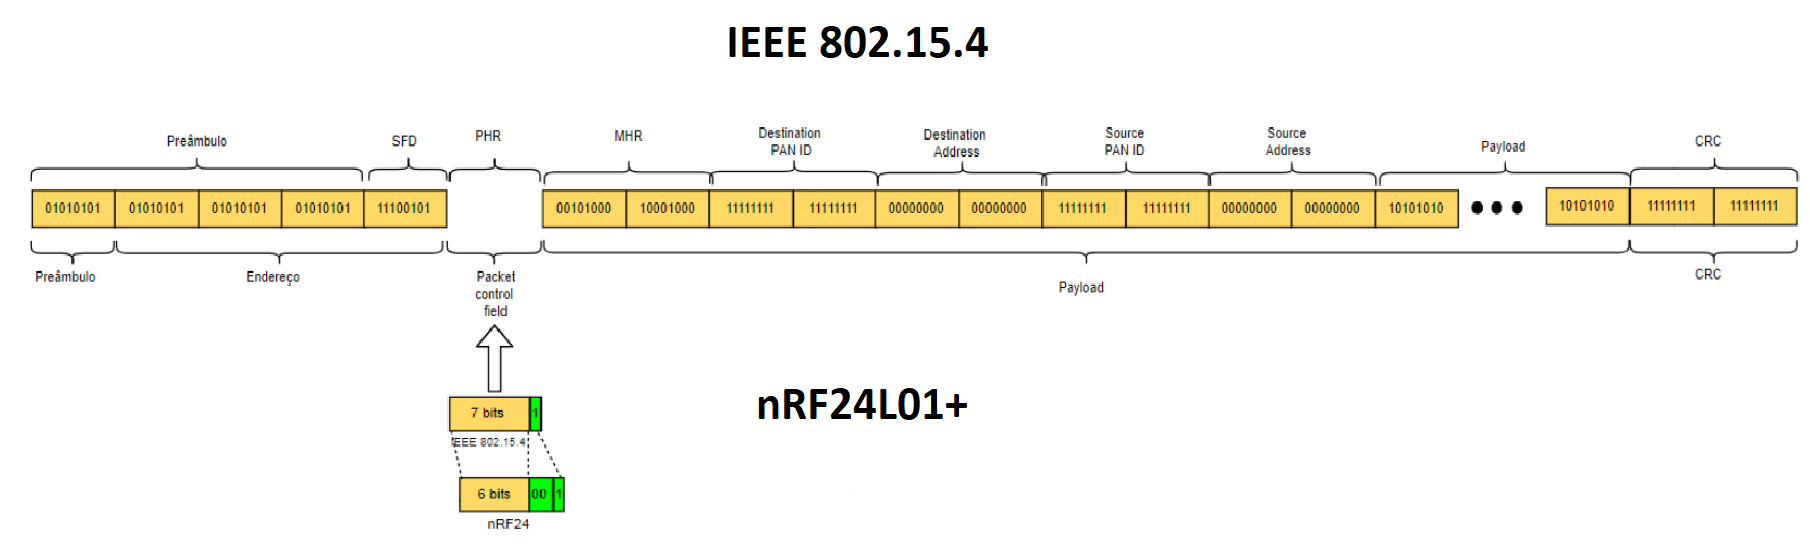
\includegraphics[width=1\textwidth]{Figuras/pacote_final.PNG}   
	\caption{Estrutura do pacote utilizado pelo projeto.}
	\label{fig:figura80}
\end{figure}

\paragraph{} Para que a adaptação representada pela figura \ref{fig:figura80} fosse possível, o nRF24L01+ precisou ser ter 4 bytes de endereço. Assim sendo, os campos PHR do IEEE 802.15.4 e o \textit{Packet Control Field} do nRF24L01+ se encontram no mesmo byte do pacote,  possibilitando que o \textit{payload} dinâmico tenha o mesmo tamanho em ambas configurações. A maior dificuldade encontrada nessa etapa foi com relação os 9 bits do \textit{Packet Control Field} que poderiam vir a dessincronizar o octeto. Para que tal não acontecesse, foi feita a expansão do campo de tamanho do nRF24L01+ para 7 bits e a compressão dos 2 bits de identificação, para que juntamente com o bit de não ACK, se tornassem apenas 1 bit. 

%\paragraph{} USRP

\paragraph{} Para gerenciar as diversas aplicações que estão sendo hospedados no microcontrolador foi utilizado um sistema operacional de tempo real, mantido pela Amazon de código aberto FreeRTOS. Cada aplicação recebe uma \textit{thread} de sistema, que gerencia o paralelismo de execução, bem como as dependências de hardware, além do uso de memória de cada aplicação. Foi utilizada também, a biblioteca de \textit{socket} do sistema operacional no interfaceamento da aplicação do servidor HTTP.  

\paragraph{} Os pacotes transmitidos foram monitorados através de uma USRP (um dispositivo RDS genérico programável) e, de um programa de linguagem gráfica G, em ambiente \textit{LabView}. Esses recursos são importantes, na medida em que monitoram o espectro RF, demodulam e decodificam os pacotes, de acordo com o protocolo IEEE 802.15.4. Vale ressaltar, que os sinais RF no canal selecionado serviram para depurar o funcionamento da rede. 

\paragraph{} Por fim, todos os códigos utilizados no desenvolvimento deste projeto foram colocados em domínio público no repositório AdHocIME git, disponível no site github.com.

%

%Foram realizados os seguintes procedimentos para se alcançar os objetivos do projeto: programação em linguagem C, para fazer a comunicação do microcontrolador com o computador via \textit{ethernet} sobre USB, recepção de pacotes enviados do nRF24L01+ por um USRP

%Dessa forma o produto final deste projeto, irá fornecer uma base para a realização da comunicação entre VANTs em uma rede Ad Hoc.

%O objetivo desse projeto é a montagem de uma rede Ad Hoc com microcontroladores que se comunicam através de um rádio RF. Para a conclusão deste objetivo, essa rede deve ser capaz de incorporar, ou excluir, dispositivos, ao se aproximarem, ou se afastarem da rede.  